\chapter{Tracking of Charged Particles}
\label{c:charged.track}

\bmad can track both charged particles and X-rays. This chapter deals
with charged particles and X-rays are handled in
chapter~\sref{c:xray.track}.

For tracking and transfer map calculations (here generically called
``tracking''), \bmad has various methods that can be applied to a
given element (Cf. Chapter~\sref{c:methods}). This chapter discusses
the \vn{bmad_standard} calculation that is the default for almost all
element types and the \vn{symp_lie_bmad} calculation that does
symplectic integration.

Generally, it will be assumed that tracking is in the forward direction.

%-----------------------------------------------------------------
\section{Relative Versus Absolute Time Tracking}
\label{s:rf.time}

\index{relative time tracking}\index{absolute time tracking}
\index{lcavity}\index{rfcavity}\index{em_field}
Unlike other elements, the kick given a particle going through an
\vn{lcavity}, \vn{rfcavity}, or possibly an \vn{em_field} element
depends upon the time that the particle enters the element relative to
some ``RF clock''. \bmad has two modes for calculating this time
called ``\vn{relative time tracking}'' and ``\vn{absolute time
tracking}''. The switch to set the type of tracking for a lattice is
\vn{parameter[absolute_time_tracking]} (\sref{s:param}).

The phase of the RF, $\phi_\text{rf}$, is determined by
\Begineq
  \phi_\text{rf} = \phi_\text{t} + \phi_\text{ref}
\Endeq
where $\phi_\text{t}$ is the part of the phase that depends upon
the time $t$ and $\phi_\text{ref}$ is a fixed phase offset (generally set
in the lattice file) and independent of the particle coordinates.

With \vn{relative time tracking}, which \bmad uses by default, the
value of $\phi_\text{t}$ at the entrance to an element is determined
by by the phase space $z$ coordinate (\sref{s:phase.space}):
\Begineq
  \phi_\text{t}(s) = \frac{-z(s) \, f_\text{rf}}{(\beta \, c)}
  = f_\text{rf} \, (t(s) - t_0(s))
\Endeq
where $f_\text{rf}$ is the RF frequency, and $t_0$ is the reference
time (\sref{s:phase.space}).

With \vn{absolute time tracking}, the RF phase at the entrance to the
cavity is determined by
\Begineq
  \phi_\text{t}(s) = f_\text{rf} \, (t(s) - t_\text{e0})
\Endeq
where $t_\text{e0}$ is the \vn{element reference time}. The element
reference time is, by definition, equal to $t_{0}(s)$ when $s$ is the
distance from the beginning of the lattice to the entrance of the RF
element. 

To understand the distinction between $t_0$ and $t_\text{e0}$,
consider a particle traveling on the reference orbit along side the
reference particle in a circular ring with one RF cavity. This
particle always has $z = 0$ and thus, with \vn{relative time
tracking}, $\phi_t$ will always be zero at the entrance to the cavity.
With \vn{absolute time tracking}, the particle, on the first turn,
will have $\phi_t$ equal to zero. However, on subsequent turns the
phase will increase by $f_\text{rf} \, t_\text{C}$ on each turn where
$t_\text{C}$ is the revolution time. If $f_\text{rf}$ is some multiple
of the revolution harmonic, the RF phase with absolute vs relative
time tracking will be some multiple of $2 \, \pi$ and thus RF kick
given the particle will be the same in both cases. However, if the RF
frequency is not some multiple of the revolution harmonic, there will
be a difference in the RF kicks (except for the kick on the first
turn).

There are advantages and disadvantages to using either relative or
absolute time tracking. Absolute time tracking is more correct since
RF cavities are in reality synced to some clock. The problem with
absolute time tracking is that the transfer map through the cavity is
now a function of time and therefore is a function of $z$ and the turn
number.  This complicates lattice analysis. For example, standard
element transfer maps use phase space coordinates so with absolute
time tracking, one has a different map for each turn.

With relative time tracking the transfer map problem is swept under
the rug. The penalty for using relative time tracking is that results
can be unphysical. For example, the closed orbit is essentially
independent of the RF frequency. From a different angle this can be
viewed as a good feature since if one is only interested in, say,
calculating the Twiss parameters, it can be an annoyance to have to
worry that the ring one has constructed have a length that is exactly
conmensurate with the RF frequency and it is potentially confusing to
see non-zero closed orbits when one is not expecting it.

The above discussion is limited to the cavity fundamental mode.
Long-range wake fields, on the other hand, cannot be synchronized to
the $z$ coordinate since, in general, their frequencies are not
commensurate with the fundamental mode frequency. For simulating the
long-range wakes, the kick is thus, by necessity, tied to the absolute
time. The exception is that a wake associated with the fundamental
mode (that is, has the same frequency as the fundamental mode) will
always use relative time if the fundamental is using relative time and
vice versa.

Do not confuse absolute time tracking with the \vn{time_runge_kutta}
tracking method (\sref{s:tkm}). The \vn{time_runge_kutta} method uses
time as the independent variable instead of $z$. Absolute time
tracking just means that the RF phase is dependent upon the time
instead of $z$. It is perfectly possible to use absolute time
tracking with code that uses $z$ as the independent variable.

%-------------------------------------------------------------------------
%-------------------------------------------------------------------------
\section{Element Coordinate System}
\label{s:ele.coords}

\index{element coordinates}
The general procedure for tracking through an element makes use of
\vn{element reference} coordinates (also called just \vn{element}
coordinates). Without any offsets, pitches or tilt (\sref{s:offset}), henceforth
called ``misalignments'', the \vn{element} coordinates are the same
as the \vn{laboratory reference} coordinates (or simply \vn{laboratory}
coordinates) (\sref{s:ref}). The \vn{element} coordinates stay fixed
relative to the element. Therefore, if the element is misaligned, the
\vn{element coordinates} will follow as the element shifts in the
laboratory frame as shown in \fig{f:ele.coord}.

Tracking a particle through an element is a three step process:
\begin{enumerate}
\item
At the entrance end of the element, transform from the \vn{laboratory}
coordinates to the entrance \vn{element} coordinates.
\item
Track through the element ignoring any misalignments. 
\item
At the exit end of the element, transform from the exit \vn{element}
reference frame to the \vn{laboratory} reference frame.
\end{enumerate}

The transformation between \vn{laboratory} and \vn{element} reference
frames will depend upon whether the element is straight or not. In
any case, it is assumed that pitches are small so that second order
terms can be ignored.

%-------------------------------------------------------------------------

\begin{figure}[tb]
  \centering
  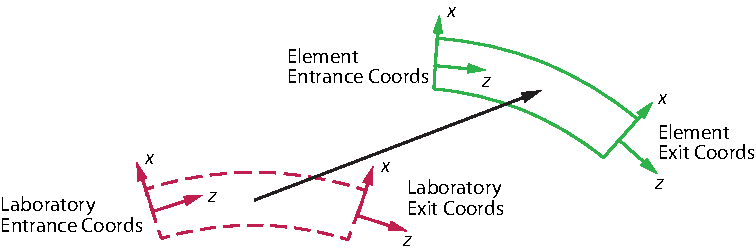
\includegraphics[width=5in]{coord-offset.pdf}
  \caption[Element Coordinate System.]
  {
\vn{Element} coordinates are coordinates attached to the physical
element (solid green outline). The \vn{laboratory} coordinates are
fixed at the nominal position of the element (red dashed outline).
  }
  \label{f:ele.coord}.
\end{figure}

%-------------------------------------------------------------------------
\subsection{Transform from Laboratory Entrance to Element Coordinates for Straight Elements}

The transformation from the laboratory coordinates to element
coordinates for an element that has a straight reference trajectory
through it is a two step process.
\begin{enumerate}
\setlength{\itemsep}{0pt}
\item
Track as in a drift a distance \vn{z_offset_tot}.
\item
Apply offsets and pitches
\vspace{-1ex}
\begin{align}
  x_1    &= x_0 - x_{\text{off}} + \frac{L}{2} \, x'_{pitch} \CRNO
  p_{x1} &= p_{x0} - (1 + p_{z0}) \, x'_{pitch} \CRNO
  y_1    &= y_0 - y_{\text{off}} + \frac{L}{2} \, y'_{pitch} \\
  p_{y1} &= p_{x0} - (1 + p_{z0}) \, y'_{pitch} \CRNO
  z_1    &= z_0 + x'_{pitch} \, x_1 + y'_{pitch} \, y_1 - 
    \frac{L}{4} (x^{\prime2}_{pitch} + y^{\prime2}_{pitch}) \nonumber
\end{align}
where $x'_{pitch}$ and $y'_{pitch}$ are the \vn{x_pitch_tot} and
\vn{y_pitch_tot} attributes of the element (\sref{s:offset}), and
$x_{\text{off}}$, and $y_{\text{off}}$ are the \vn{x_offset_tot} and
\vn{y_offset_tot} attributes.
Notice that $z_1$ is written in terms of $x_1$ and $y_1$
\item
Apply the tilt $\theta_t$ (\vn{tilt_tot})
\vspace{-1ex}
\begin{align}
  x_2    &=  x_1    \, \cos\theta_t + y_1    \, \sin\theta_t \CRNO
  p_{x2} &=  p_{x1} \, \cos\theta_t + p_{y1} \, \sin\theta_t \CRNO
  y_2    &= -x_1    \, \sin\theta_t + y_1    \, \cos\theta_t \\
  p_{y2} &= -p_{x1} \, \sin\theta_t + p_{y1} \, \cos\theta_t \nonumber
\end{align}
\end{enumerate}

%-------------------------------------------------------------------------
\subsection{Transform from Laboratory Entrance to Element Coordinates for Bend Elements}

Let $\bfr_c$ be the displacement of the bend at the bend center (where
offsets are specified \sref{s:offset}).

The rotation matrix $\bfS_c$ transforming
from the center of the bend (where the misalignments are defined) to the
entrance face of the bend is
\begin{align}
  \bfS_c &= \bfR_{z}^{-1} (\theta_t) \, \bfR_{y} (\alpha_b/2) \, \bfR_{z} (\theta_t) \\
\end{align}
where $\bfR_{z}$ and $\bfR_{y}$ are given by \Eqs{wtt0t},
$\theta_t$ is the \vn{ref_tilt} attribute of the bend and $\alpha_b$
is the bend \vn{angle}.

In the laboratory entrance coordinates, the pitches and offset are
\begin{align}
  \bfW &= \bfS \, 
    \begin{pmatrix}
      -y'_{pitch} \\ x'_{pitch} \\ 0
    \end{pmatrix} \\
  \bfV &= \bfS \, 
    \begin{pmatrix}
      x_{\text{off}} \\ y_{\text{off}} \\ z_{\text{off}} + 
    \end{pmatrix} +
    \bfS \, \bfL_c - \bfL_c
\end{align}
where the offset vector $\bfL_c$ is
\Begineq
  \bfL_c = \bfR_{z}(\theta_t) \,
      \begin{pmatrix}
        2 \, \rho \, \sin^2 (\alpha_b / 2) \\ 0 \\ -\rho \, \sin(\alpha_b / 2)
      \end{pmatrix}
\Endeq

The transformation to element coordinates is then
\begin{enumerate}
\setlength{\itemsep}{0pt}
\item
\begin{align}
  x_1    &= x_0 - \bfV(1) \CRNO
  p_{x1} &= p_{x0} - \bfW(1) \, (1 + p_{z0}) \CRNO
  y_1    &= y_0 - \bfV(2) \\
  p_{y1} &= p_{x0} + \bfW(2) \, (1 + p_{z0}) \CRNO
  z_1    &= z_0 + \bfW(2) \, x_0 - \bfW(1) \, y_0 \nonumber
\end{align}
\item
Track as in a drift a distance $\bfV(3)$.
\item
Apply the non-reference shifting tilt $\theta_t$ (\vn{tilt_tot})
\vspace{-1ex}
\begin{align}
  x_2    &=  x_1    \, \cos\theta_t + y_1    \, \sin\theta_t \CRNO
  p_{x2} &=  p_{x1} \, \cos\theta_t + p_{y1} \, \sin\theta_t \CRNO
  y_2    &= -x_1    \, \sin\theta_t + y_1    \, \cos\theta_t \\
  p_{y2} &= -p_{x1} \, \sin\theta_t + p_{y1} \, \cos\theta_t \nonumber
\end{align}
\end{enumerate}

%-------------------------------------------------------------------------
\subsection{Transform from Element Exit to Laboratory Coordinate for Straight Elements}

The back transformation from element to laboratory coordinates is
accomplished by the transformation
\begin{enumerate}
\setlength{\itemsep}{0pt}
\item
Apply tilt $\theta_t$
\vspace{-1ex}
\begin{align}
  x_1    &=  x_0    \, \cos\theta_t - y_0    \, \sin\theta_t \CRNO
  p_{x1} &=  p_{x0} \, \cos\theta_t - p_{y0} \, \sin\theta_t \CRNO
  y_1    &=  x_0    \, \sin\theta_t + y_0    \, \cos\theta_t \\
  p_{y1} &=  p_{x0} \, \sin\theta_t + p_{y0} \, \cos\theta_t \nonumber
\end{align}
\item
Apply offsets and pitches
\vspace{-1ex}
\begin{align}
  x_2    &= x_1 + x_{\text{off}} + \frac{L}{2} x'_{pitch}     \CRNO
  p_{x2} &= p_{x1} + (1 + p_{z1}) \, x'_{pitch}        \CRNO
  y_2    &= y_1 + y_{\text{off}} + \frac{L}{2} y'_{pitch}     \\
  p_{y2} &= p_{x1} + (1 + p_{z1}) \, y'_{pitch}        \CRNO
  z_2    &= z_1 + x'_{pitch} \, x_1 + y'_{pitch} \, y_1 - 
    \frac{L}{4} (x^{\prime2}_{pitch} + y^{\prime2}_{pitch})      \nonumber
\end{align}
\item
Track as in a drift a distance \vn{-z_offset_tot}.
\end{enumerate}

%-------------------------------------------------------------------------
\subsection{Transform from Element Exit to Laboratory Coordinate for Bend Elements}

The back transformation from element to laboratory coordinates is
accomplished by the transformation
\begin{enumerate}
\setlength{\itemsep}{0pt}
\item
Apply non-reference shifting tilt $\theta_t$
\vspace{-1ex}
\begin{align}
  x_1    &=  x_0    \, \cos\theta_t - y_0    \, \sin\theta_t \CRNO
  p_{x1} &=  p_{x0} \, \cos\theta_t - p_{y0} \, \sin\theta_t \CRNO
  y_1    &=  x_0    \, \sin\theta_t + y_0    \, \cos\theta_t \\
  p_{y1} &=  p_{x0} \, \sin\theta_t + p_{y0} \, \cos\theta_t \nonumber
\end{align}
\item
Apply offsets and pitches
\vspace{-1ex}
\begin{align}
  x_1    &= x_0 + \bfV(1) \CRNO
  p_{x1} &= p_{x0} + \bfW(1) \, (1 + p_{z0}) \CRNO
  y_1    &= y_0 + \bfV(2) \\
  p_{y1} &= p_{x0} - \bfW(2) \, (1 + p_{z0}) \CRNO
  z_1    &= z_0 - \bfW(2) \, x_0 + \bfW(1) \, y_0 \nonumber
\end{align}
\item
Track as in a drift a distance \vn{-z_offset_tot}.
\end{enumerate}

%-------------------------------------------------------------------------
\section{Hamiltonian}
\label{s:mag.hamiltonian}
The time dependent Hamiltonian $H_t$ in the curvilinear coordinate system shown
in \fig{f:local.coords} is (\cite{b:ruth})
\Begineq
  H_t = \wt\psi + \left[ \left( \frac{p_s - a_s}{1 + g\, x} \right)^2 + \wt m^2 + 
  (p_x - a_x)^2 + (p_y - a_y)^2 \right]^{1/2}
\Endeq
where $(p_x, p_y, p_s/(1+gx))$ are the momentum normalized by $P_0$,
$\rho$ being the local radius of curvature of the reference particle,
and $\wt m$, $\Bf a$ and $\wt\psi$ are the normalized mass, vector, and scalar
potentials:
\Begineq
  \wt m = \frac{m \, c^2}{c \, P_0} \qquad
  \left( a_x, a_y, \frac{a_s}{1+g \, x} \right) = \frac{q \, \Bf A}{P_0 \, c} \qquad 
  \wt\psi(x,y,z) = \frac{q \, \psi}{P_0 \, c}
  \label{mmccp}
\Endeq
In terms of the normalized velocities $\beta_x$, $\beta_y$, the canonical momentum are
\Begineq
  p_x = \frac{m \, c^2}{P_0 \, c} \, \beta_x + a_x, \qquad 
  p_y = \frac{m \, c^2}{P_0 \, c} \, \beta_y + a_y
  \label{pmc2pc}
\Endeq

The $s$-dependent Hamiltonian is obtained from $H_t$ by solving for
$-p_s$ and using a contact transformation to convert to \bmad
coordinates (\sref{s:phase.space}). For particles propagating in the
positive $s$ direction, the $s$-dependent Hamiltonian is, assuming
$\wt\psi$ is zero
\Begineq
  H \equiv H_s = -(1 + g \, x) \sqrt{(1 + p_z)^2 - (p_x - a_x)^2 - (p_y - a_y)^2} - 
  a_s + \frac{1}{\beta_0} \, \sqrt{(1+p_z)^2 + \wt m^2}
  \label{h1gx1}
\Endeq
where $\beta_0$ is the reference velocity and the equality $(1 +
p_z)^2 = (E/c\, P_0)^2 - \wt m^2$ has been used. The last term on the
RHS of \Eq{h1gx1} accounts for the fact that the \bmad canonical $z$
(\Eq{zbctt}) has an ``extra'' term $\beta \, c \, t_0$ so that \bmad
canonical $z$ is with respect to the reference particle's $z$.

The equations of motion are
\begin{equation}
  \frac{dq_i}{ds} = \frac{\partial H}{\partial p_i} \qquad
  \frac{dp_i}{ds} = -\frac{\partial H}{\partial q_i}
  \label{rshp}
\end{equation}

\label{paraxial approximation} 
Without an electric field, $\psi$ is zero. Assuming a non-curved
coordinate system ($g = 0$), and using the paraxial approximation
(\sref{s:phase.space}), \Eq{h1gx1} becomes
\Begineq
  H = \frac{(p_x - a_x)^2}{2 (1 + p_z)} + \frac{(p_y - a_y)^2}{2 (1 + p_z)} - 
  (1 + g \, x) \, (1 + p_z) - a_s +   \frac{1}{\beta_0} \, \sqrt{(1+p_z)^2 + \wt m^2}
  \label{hpapa}
\Endeq

Once the transverse trajectory has been calculated, the longitudinal position
$z_2$ at the exit end of an element is obtained from symplectic
integration of \Eq{hpapa}
\Begineq
  z_2 = z_1 - \frac{1}{2 (1 + p_{z1})^2} \int \! ds \, 
  \left[ (p_x - a_x)^2 + (p_y - a_y)^2 \right] - \int \! ds \, g \, x
  \label{zz121p}
\Endeq
where $z_1$ is the longitudinal position at the entrance end of the element.
Using the equations of motion \Eqs{rshp} this can also be rewritten as
\Begineq
  z_2 = z_1 - \frac{1}{2} \int \! ds \, 
  \left[ \left( \frac{dx}{ds} \right)^2 + \left( \frac{dy}{ds} \right)^2 \right] - 
  \int \! ds \, g \, x
  \label{zz12sx}
\Endeq

For some elements, \vn{bmad_standard} uses a truncated Taylor map for
tracking.  For elements without electric fields where the particle
energy is a constant, the transfer map for a given coordinate $r_i$
may be expanded in a Taylor series
\Begineq
  r_{i,2} \rightarrow m_i + \sum_{j = 1}^4 m_{ij} \, r_{j,1} + 
  \sum_{j = 1}^4 \sum_{k = j}^4 m_{ijk} \, r_{j,1} \, r_{k,1} + \ldots
\Endeq
where the map coefficients $m_{ij\cdots}$ are functions of $p_z$.  For
linear elements, the transfer map is linear for the transverse
coordinates and quadratic for $r_i = z$.

Assuming mid--plane symmetry of the magnetic field, so
that $a_x$ and $a_y$ can be set to zero\cite{b:madphysics}, The vector
potential up to second order is (cf.~\Eq{byx0b})
\Begineq
  a_s = -k_0 \left( x - \frac{g \, x^2}{2 (1 + g\, x)} \right) -
  \frac{1}{2} k_1 \left( x^2 - y^2 \right)
  \label{akxgx}
\Endeq

For backwards propagation, where particle are traveling in the $-\Bf
s$ direction and where $p_s$ is negative, solving for $p_s$ involves
using a different part of the square root branch. There is also an
overall negative sign coming from switching from using $s$ as the
independent variable to $\wt s \equiv -s$ as the independent
variable. the Hamiltonian $H_{\wt s}$ is then
\Begineq
  H_{\wt s} = -(1 + g \, x) \sqrt{(1 + p_z)^2 - (p_x - a_x)^2 - (p_y - a_y)^2} + 
  a_s + \frac{1}{\beta_0} \, \sqrt{(1+p_z)^2 + \wt m^2}
\Endeq

%---------------------------------------------------------------------------------
%---------------------------------------------------------------------------------
\section{Symplectic Integration}
\label{s:symp.track}
\index{symplectic integration}

Using \Eq{hpapa} the Hamiltonian is written in the form
\Begineq
  H = H_x + H_y + H_z
\Endeq
where
\begin{equation}
  H_x = \frac{(p_x - a_x)^2}{2 (1 + \delta)}, \qquad
  H_y = \frac{(p_y - a_y)^2}{2 (1 + \delta)}, \qquad
  H_s = - a_s 
\end{equation}

For tracking, the element is broken up into a number of slices set by
the element's \vn{ds_step} attribute. For each slice, the tracking
uses a quadratic symplectic integrator $I$:
\Begineq
  I = T_{s/2} \; I_{x/2} \; I_{y/2} \; I_s \; I_{y/2} \; I_{x/2} \; T_{s/2}
\Endeq
$T_{s/2}$ is just a translation of the $s$ variable:
\Begineq
  s \rightarrow s + \frac{ds}{2}
\Endeq
And the other integrator components are
\begin{align}
  I_{x/2} &= \exp \left( : -\frac{ds}{2} H_x : \right) \CRNO
  I_{y/2} &= \exp \left( : -\frac{ds}{2} H_y : \right) \\
  I_{s}   &= \exp \left( : -ds \, H_s : \right) \nonumber
\end{align}
The evaluation of $I_{x/2}$ and $I_{y/2}$ is tricky since it involves both transverse
position and momentum variables. The trick is to split the integration into three parts.
For $I_{x/2}$ this is
\begin{align}
  I_{x/2} &= \exp \left( : -\frac{ds}{2} \frac{(p_x - A_x)^2}{2 (1 + \delta)} : \right) \CRNO
  &= \exp \left( : -\int A_x \, dx : \right) \,
     \exp \left( : -\frac{ds}{2} \frac{p_x^2}{2 (1 + \delta)} : \right) \,
     \exp \left( : \int A_x \, dx : \right)
  \label{ids2}
\end{align}
With an analogous expression for $I_{y/2}$.

\index{quadrupole}\index{sextupole}\index{wiggler}
For magnetic elements that do not have longitudinal fields
(quadrupoles, sextupoles, etc.), $a_x$ and $a_y$ can be taken to be
zero (cf.~\Eq{akxgx}).

\index{lcavity}\index{rfcavity}
For \vn{lcavity} and \vn{rfcavity} elements, the vector potential is computed from
\Eq{aiew}.

%-----------------------------------------------------------------   
\section{Spin Dynamics}   
\label{s:spin.dyn}
\index{spin|hyperbf}   

\textit{\large [Spin dynamics initially developed by Jeff Smith]}

The classical spin vector $\Bf S$ is described in the local reference
frame (\sref{s:ref}) by a modified Thomas-Bargmann-Michel-Telegdi
(T-BMT) equation\cite{b:spin}
\Begineq
  \frac{\mathrm{d}}{\mathrm{d}s} \Bf S = 
  \left\{ \frac{(1+\Bf r_t \dotproduct \bfg)}{c \, \beta_z} \, 
  \left( {\pmb\Omega}_{BMT} + {\pmb\Omega}_{EDM} \right) - 
  \bfg \times \bfhat z \right\} \times \mathbf{S}
  \label{tbmt}
\Endeq
where $\bfg$ is the bend curvature function which points away from the center of curvature
of the particle's reference orbit (see \fig{f:local.coords}), $\Bf r_t = (x, y)$ are the
transverse coordinates, $c \, \beta_z$ is the longitudinal component of the velocity, and
$\bfhat z$ is the unit vector in the $z$-direction. $\pmb\Omega_{BMT}$ is the usual T-BMT
precession vector due to the particle's magnetic moment and $\pmb\Omega_{EDM}$ is the
precession vector due to a finite electric dipole moment (EDM) \cite{b:silenko}
\begin{align}
  {\pmb\Omega}_{BMT} (\mathbf{r,P},t) &= 
    - \frac{q}{m \, c} \left[ 
    \left(\frac{1}{\gamma} + G \right) \, c \, \Bf B -
    \frac{G \, \gamma \, c}{1 + \gamma} \, ( \bfbeta \dotproduct \Bf B ) \, \bfbeta -
    \left( G + \frac{1}{1 + \gamma} \right) \, \mathbf{\bfbeta \times  E} 
    \right] \\
  &= - \frac{q}{m \, c} \left[ 
    \left( \frac{1}{\gamma} + G \right) \, c \, \Bf B_{\perp} +
    \frac{(1 + G) \, c}{\gamma} \, \Bf B_\parallel -
    \left( G + \frac{1}{1 + \gamma} \right) \mathbf{\bfbeta \times E} 
    \right] \nonumber
\end{align}
and
\Begineq
  {\pmb\Omega}_{EDM} (\mathbf{r,P},t) = 
  - \frac{q \, \eta}{2 \, m \, c} \left[
  \Bf E - \frac{\gamma}{1 + \gamma} \, 
  ( \bfbeta \dotproduct \Bf E ) \, \bfbeta +
  c \, \mathbf{\bfbeta \times B}
  \right]
\Endeq
Here $\Bf E (\Bf r ,t)$ and $\Bf B (\Bf r ,t)$ are the electric and magnetic fields, $\Bf
B_\perp$ and $\Bf B_\parallel$ are the components perpendicular and parallel to the
momentum, $\gamma$ is the particle's relativistic gamma factor, $q$, $m$, and $\eta$ are
the particle's charge, mass, and magnetic_moment, $\bfbeta$ is the normalized
velocity, and $G = (g-2)/2$ is the particle's anomalous gyro-magnetic g-factor (values
given in Table~\ref{t:constants}).
   
It is more efficient to use the SU(2) representation rather than SO(3) when   
describing rotations of spin. In the SU(2) representation, a spin $\Bf s$ is   
written as a spinor $\Psi = \left( \psi_{1}, \psi_{2} \right)^{T}$ where   
$\psi_{1,2}$ are complex numbers. The conversion between SU(2) and SO(3) is  
\Begineq  
  \Bf S = \Psi^{\dagger} \Bf {\bfsig} \, \Psi 
  \qquad \longleftrightarrow \qquad
  \Psi  = \frac{e^{i \xi}}{\sqrt{2 \left(P+s_{3}\right)}}   
     \begin{pmatrix} P+s_{3} \\ s_{1}+i s_{2} \end{pmatrix}   
  \Endeq  
Where $\xi$ is an unmeasureable phase factor, and $P$ is the polarization. $P = 1$ for a single
particle. Also ${\bfsig} = (\sigma_x, \sigma_y, \sigma_z)$ are the three Pauli matrices
\Begineq
  \sigma_x = \begin{pmatrix} 0 &  1 \\ 1 &  0 \end{pmatrix}, \qquad
  \sigma_y = \begin{pmatrix} 0 & -i \\ i &  0 \end{pmatrix}, \qquad
  \sigma_z = \begin{pmatrix} 1 &  0 \\ 0 & -1 \end{pmatrix}
\Endeq
In polar coordinates
\Begineq   
  \Psi = \begin{pmatrix} \psi_{1} \\ \psi_{2} \end{pmatrix}
       = \sqrt{P} \, e^{i \xi}
         \begin{pmatrix} 
            \cos \frac{\theta}{2} \\   
            e^{i \phi} \, \sin \frac{\theta}{2}
         \end{pmatrix}
  \qquad \longleftrightarrow \qquad
  \Bf S = P \, \begin{pmatrix} \sin \theta \cos \phi \\   
                          \sin \theta \sin \phi \\   
                          \cos \theta \end{pmatrix}
  \label{pp1p2}
\Endeq
Due to the unitarity of the spin vector,   
$|\psi_{1}|^{2} + |\psi_{2}|^{2} = P$.
The spinor eigenvectors along the $x$, $y$ and $z$ axes are
\begin{align}
   \Psi_{x+} &= \frac{1}{\sqrt{2}} \, \begin{pmatrix} 1 \\ 1 \end{pmatrix} \, , 
  &\Psi_{x-} &= \frac{1}{\sqrt{2}} \, \begin{pmatrix} 1 \\ -1 \end{pmatrix} \, , \CRNO
   \Psi_{y+} &= \frac{1}{\sqrt{2}} \, \begin{pmatrix} 1 \\ i \end{pmatrix} \, , 
  &\Psi_{y-} &= \frac{1}{\sqrt{2}} \, \begin{pmatrix} 1 \\ -i \end{pmatrix} \, , \\
   \Psi_{z+} &=                       \begin{pmatrix} 1 \\ 0 \end{pmatrix} \, , 
  &\Psi_{z-} &=                       \begin{pmatrix} 0 \\ -1 \end{pmatrix} \, . \nonumber
\end{align}

In spinor notation, the T-BMT equation can be written as
  \Begineq   
    \frac{\mathrm{d}}{\mathrm{d} t} \Psi = - \frac{i}{2} \left( \bfsig \dotproduct   
    {\pmb\Omega} \right) \Psi = -\frac{i}{2} \begin{pmatrix}
    \Omega_z & \Omega_x - i \, \Omega_y \\
    \Omega_x + i \, \Omega_y & -\Omega_z \end{pmatrix}
    \Psi
  \Endeq   
The solution leads to a rotation of the spin vector by an angle   
$\alpha$ around a unit vector $\bfhat n$ represented as   
  \begin{align}   
    \Psi_f &= \exp \left[ -i \frac{\alpha}{2} \bfhat n \dotproduct \bfsig \right] \Psi_i \CRNO
         &= \left[ \cos \left( \frac{\alpha}{2} \right) \, \Bf 1_{2} - 
            i \, (\bfhat n \dotproduct \bfsig) \, \sin \left( \frac{\alpha}{2} \right) \right] \Psi_i \\
         &= \Bf A \Psi_i. \nonumber
  \end{align}   
where $\Psi_i$ is the initial spin state, $\Psi_f$ is the final spin state, and $\Bf A$,
which describes the spin transport, is the SU(2) matrix representation of the quaternian
$(a_0, \Bf a) = (\cos(\alpha/2), -\sin(\alpha/2) \, \bfhat n)$. $\Bf A$ has the
normalization condition $a_{0}^{2} + \boldsymbol{a}^{2} = 1$. Thus the three components
$\boldsymbol{a} = \left(a_{1}, a_{2}, a_{3}\right)$ completely describe $\Bf A$. 

With spinors, the matrix representation of the observable $S_{\Bf u}$
corresponding to the measurement of the spin along the unit vector
$\Bf u$ is
\begin{align}
  S_{\Bf u} &\equiv \frac{\hbar}{2} \, \bfsig \dotproduct \Bf u \\   
            &= \frac{\hbar}{2} 
                   \begin{pmatrix} 
                     u_z            & u_x - i \, u_y \\
                     u_x + i \, u_y & u_z
                   \end{pmatrix}
\end{align}
The expectation value of this operator, $\Psi^\dagger \, \Bf S_u \,
\Psi$, representing the spin of a particle, satisfies the equation of
motion of a classical spin vector in the particle's instantaneous rest
frame.

For a distribution of spins, the polarization $P_s$ along the unit
vector $\Bf u$ is defined as the absolute value of the average
expectation value of the spin over all N particles times
$\frac{2}{\hbar}$,
  \Begineq
    P_s = \frac{2}{\hbar} \frac{1}{N} \sum_{j=1}^{N} \Psi_j^\dagger S_{\Bf u} \Psi_j
  \Endeq  

See \S~\sref{s:spin.hard.fringe} for formulas for tracking a spin through a multipole
fring field.

%---------------------------------------------------------------------------------
%---------------------------------------------------------------------------------
\section{Fringe Fields}
\label{s:multi.fringe.std}
\index{fringe!multipole}

The fringe field kick is divided into two pieces. 
The first piece is called the \vn{hard edge} fringe kick and is the kick in the limit
that the longitudinal extent of the fringe is zero. The second piece is the 
\vn{soft edge} fringe kick which is the fringe kick with the fringe having a finite
longitudinal extent minus the hard edge fringe kick. That is
\begin{example}
  fringe kick = hard fringe kick + soft fringe kick
\end{example}
The advantage of separating the fringe kick in this way is that the hard fringe can
be used without having to know anything about the longitudinal extent of the fringe
field. In many cases, this is a good enough approximation. 

%---------------------------------------------------------------------------------
\subsection{Bend Soft Edge Fringe Map}


\bmad defines the bend soft edge map in terms of the field integral
$F_{H1}$ for the entrance end and $F_{H2}$ for the exit end given by
(see \Eq{fsbbb})
\Begineq
  F_{H1} \equiv F_{int} \, H_{gap} = \int_{pole} \! \! ds \, \frac{B_y(s) \, (B_{y0} - B_y(s))}
  {2 \, B_{y0}^2}
\Endeq
With a similar equation for $F_{H2}$.
The soft edge map is then
\begin{align}
  x_2 &=  x_1 + c_1 \, p_z \CRNO
  p_{y2} &= p_{y1} + c_2 \, y_1 - c_3 \, y_1^3 \\
  z_2 &= z_1 + \frac{1}{1 + p_{z1}} \, \left( 
    c_1 \, p_{x1} + \frac{1}{2} \, c_2 \, y_1^2 -\frac{1}{4} \, c_3 \, y_1^4 \right)
    \nonumber
\end{align}
For the entrance face:
\Begineq
  c_1 = \frac{g_{tot} \, F_{H1}^2}{2 \, (1 + p_z)}, \qquad 
  c_2 = \frac{2 \, g_{tot}^2 \, F_{H1}}{1 + p_z}, \qquad 
  c_3 = 0
\Endeq
with \vn{g_{tot}} is the total bending strength
\Begineq
  g_{tot} = \text{g} + \text{g_err}
\Endeq
\vn{g} being the reference bend strength and \vn{g_err} being
bend the difference between the actual and reference bend strengths
(\sref{s:bend}).

For the exit face, the subsitution is made
\begin{align}
  F_{H1} &\rightarrow F_{H2} \CRNO
  g_{tot} &\rightarrow -g_{tot}
\end{align}

When the SAD bend soft edge map is used (\sref{s:fringe}), the map is
the same except that the value of $c_3$ is
\Begineq
  c_3 = \frac{8 \, g_{tot}^2}{F_{H1} \, (1 + p_z)}
\Endeq
It might seem strange that $c_3$ diverges to infinity as $F_H$ goes to
zero since naively one would expect the soft edge kick to vanish in
the hard edge limit where the fringe has no longitudinal
extent. However, in the hard edge limit, the field does not obey
Maxwell's equations. The limiting map, as $F_H$ goes to zero, has
fields that diverge to infinity and this exaplains why the full (hard
+ soft) limiting map is not the same as the hard edge map at the limit
of zero longitudinal extent.

For a \vn{sad_mult} element, the field integrals are characterized by
parameters \vn{fb1} (entrance end) and \vn{fb2} (exit end) which
correspond to the SAD \vn{fb1} and \vn{fb2} parameters. These are related
to the bend parameters by
\Begineq
  \text{fb1} = 12 \, F_{H1}, \qquad \text{fb2} = 12 \, F_{H2}
\Endeq

%---------------------------------------------------------------------------------
\subsection{Bend Hard Edge Fringe Map}

In development...

%---------------------------------------------------------------------------------
\subsection{Quadrupole Soft Edge Fringe Map}
\label{s:q.soft}

Only the quadrupole soft edge fringe is modeled in \bmad. The model is adapted 
from SAD\cite{b:sad}. The fringe map is:
\begin{align}
  x_2 &= x_1 \, e^{g_1} + g_2 \, p_{x1} \CRNO
  p_{x2} &= p_{x1} e^{-g_1} \CRNO
  y_2 &= y_1 \, e^{-g_1} - g_2 \, p_{y1} \\
  p_{y2} &= p_{y1} e^{g_1} \CRNO
  z_2 &= z_1 - 
    \left[g_1 \, x_1 \, p_{x1} + g_2 \, \left( 1 + \frac{g_1}{2} \right)
    \, e^{-g_1} \, p_{x1}^2 \right] + 
    \left[g_1 \, y_1 \, p_{y1} + g_2 \, \left( 1 - \frac{g_1}{2} \right)
    \, e^{g_1} \, p_{y1}^2 \right] \nonumber
\end{align}
where
\begin{align}
  g_1 &= K_1 \, \text{fq1} \CRNO
  g_2 &= K_1 \, \text{fq2}
\end{align}
$K_1$ is the quadrupole strength, and \vn{fq1} and \vn{fq2} are the fringe
quadrupole parameters. These parameters are related to the field integral $I_n$
via
\begin{align}
  \text{fq1} &= I_1 - \frac{1}{2} \, I_0^2 \CRNO
  \text{fq2} &= I_2 - \frac{1}{3} \, I_0^3
\end{align}
where $I_n$ is defined by
\Begineq
  I_n = \frac{1}{K_1} \, \int_{-\infty}^{\infty} \; 
    (K_1(s) - H(s-s_0) \, K_1) \, (s - s_0)^n \, ds
\Endeq
and $H(s)$ is the step function
\Begineq
  H(s) = \begin{cases}
    1   & s > 0 \\
    0   & s < 0
  \end{cases}
\Endeq
and it is assumed that the quadrupole edge is at $s_0$ and the interior is 
in the region $s > s_0$. 

The quadrupole parameters are related to the corresponding SAD parameters 
\vn{f1} and \vn{f2} via
\begin{example}
  f1 = -sign(fq1) * sqrt(24 * |fq1|)
  f2 = fq2
\end{example}
In the SAD documentation, the soft edge is called the ``linear'' fringe.

%---------------------------------------------------------------------------------
\subsection{Magnetic Multipole Hard Edge Fringe}

The magnetic multipole hard edge fringe field is modeled using the method shown in
Forest\cite{b:forest}. For the $m$\Th order multipole the Lee transform 
is (Forest Eq.~(13.29):
\begin{align}
  f_\pm &= \mp \Re \left[ \frac{(b_m + i \, a_m) \, 
    (x + i \, y)^{m+1}}{4 \, (m + 2) \, (1 + \delta)} \,
    \left\{ x \, p_x + y \, p_y + i \frac{m+3}{m+1} 
    (x \, p_x - y \, p_y) \right\} \right] \CRNO
  &\equiv \frac{p_x \, f^x + p_y \, f^y}{1 + \delta}
\end{align}
The multipole strengths $a_m$ and $b_m$ are given by \eq{bib1nb}
and the second equation defines $f^x$ and $f^y$. On the right had side of the first
equation, the minus sign is appropriate for particles entering the magnet and the
plus sign is for particle leaving the magnet.
Notice that here the multipole order $m$ is equivalent to $n-1$ in Forest's notation.

With this, the implicit multipole map is (Forest Eq.~(13.31))
\begin{align}
  x^f &= x - \frac{f^x}{1 + \delta} \CRNO
  p_x &= p_x^f - \frac{p_x^f \, \partial_x f^x + p_y^f \, \partial_x f^y}{1 + \delta} \CRNO
  y^f &= y - \frac{f_y}{1 + \delta} \\
  p_y &= p_y^f - \frac{p_x^f \, \partial_y f^x + p_y^f \, \partial_y f^y}{1 + \delta} \CRNO
  \delta^f &= \delta \CRNO
  z^f &=\frac{p_x^f \, f^x + p_y^f \, f^y}{(1 + \delta)^2} \nonumber
\end{align}

%---------------------------------------------------------------------------------
\subsection{Electrostatic Multipole Hard Edge Fringe}
\label{s:spin.hard.fringe}

The electric multipole hard edge fringe field, to lowest order, consists of just a
longitudinal field. The integrated longitudinal field at constant $(x,y)$ for the $n$\Th
order multipole is simply obtained by requireing that the curl of the field is zero.
This gives:
\Begineq
  \int E_s(x,y) \, ds = \phi_n(x,y)
\Endeq
where $\phi_n$ is given in \Eq{pbian1}. [For a magnetic multipole there is an analogous
equation.]

The effect on the spin when tracking through the fringe field of a multipole field tends
to be weak. As such, this hard edge model is sufficient.  and the spin is tracked using
the T-BMT equation (\Eq{tbmt}).

%---------------------------------------------------------------------------------
%---------------------------------------------------------------------------------
\section{BeamBeam Tracking}
\label{s:beambeam.std}
\index{beambeam}

A beam-beam element (\sref{s:bbi}) simulates the effect on a tracked
particle of an opposing beam of particles moving in the opposite
direction. The opposing beam, called the ``strong'' beam, is assumed
to be Gaussian in shape.

The strong beam is divided up into \vn{n_slice} equal charge (not
equal thickness) slices. Propagation through the strong beam involves
a kick at the charge center of each slice with drifts in between the
kicks. The kicks are calculated using the standard Bassetti--Erskine
complex error function formula\cite{b:talman}.  Even though the strong
beam can have a finite \vn{sig_z}, the length of the element is always
considered to be zero. This is achieved by adding drifts at either end
of any tracking so that the longitudinal starting point and ending
point are identical. The longitudinal $s$--position of the
\vn{BeamBeam} element is at the center of the strong bunch. For
example, with \vn{n_slice} = 2 the calculation would proceed as
follows:
\begin{enumerate}
  \item  Start with the reference particle at the center of the strong bunch.
  \item  Propagate (drift) backwards to the center of the first slice.
  \item  Apply the beam--beam kick due to the first slice.
  \item  Propagate (drift) forwards to the center of the second slice.
  \item  Apply the beam--beam kick due to the second slice.
  \item  Propagate (drift) backwards to end up with the reference particle
     at the center of the strong bunch.
\end{enumerate}

%---------------------------------------------------------------------------------
%---------------------------------------------------------------------------------
\section{Bend Element: Fringe Tracking}
\label{s:.bend.fringe.std}
\index{sbend}

The transformation for the entrance face of an \vn{sbend} is
\begin{align}
  p_{x2} &= p_{x1} + k_x \, x_1 \CRNO
  p_{y2} &= p_{y1} + k_y \, y_1
\end{align}
where
\begin{align}
  k_x &= g_{tot} \, \tan(e_1) \CRNO
  k_y &= -g_{tot} \, \tan \left[ e_1 - 2 \, |g_{tot}| \, f_{int} \,  h_{gap} \, 
    \frac{1 + \sin(e1)^2}{\cos(e_1)} \right]
\end{align}
where $g_{tot}$ is the total bending strength (design +
error). Similar equations are used for tracking the exit edge of the
bend.

%---------------------------------------------------------------------------------
%---------------------------------------------------------------------------------
\section{Bend Element: Body Tracking}
\label{s:bend.body.std}
\index{sbend}

The Hamiltonian for the body of an \vn{sbend} is
\Begineq
  H = (k_0 - g) x - g \, x \, p_z + 
  \frac{1}{2}\left( (k_1 + g \, k_0) x^2 - k_1 \, y^2 \right) +
  \frac{p_x^2 + p_y^2}{2 (1 + p_z)} 
\Endeq

This is simply solved
\begin{align}
  x_2    &= c_x \, (x - x_c) + s_x \, \frac{p_{x1}}{1 + p_{z1}} + x_c \CRNO
  p_{x2} &= \tau_x \, \om_x^2 \, \, (1 + p_{z1}) \, s_x \, (x -x_c) + c_x \, p_{x1} \CRNO
  y_2    &= c_y \, y_1 + s_y \, \frac{p_{y1}}{1 + p_{z1}} \CRNO
  p_{y2} &= \tau_y \, \om_y^2 \, \, (1 + p_{z1}) \, s_y \, y_1 + c_y \, p_{y1} \\
  z_2    &= z_1 + m_5 + m_{51} (x - x_c) + m_{52} p_{x1} + m_{511} \, (x-x_c)^2 \, + \CRNO
         &\hspace*{20ex} m_{512} \, (x-x_c) \, p_{x1} + m_{522} \, p_{x1}^2 + 
                         m_{533} \, y^2 + m_{534} \, y_1 \, p_{y1} + m_{544} \, p_{y1}^2 \CRNO
  p_{z2} &= p_{z1} \nonumber
\end{align}
where 
\begin{alignat}{2}
  k_x &= k_1 + g \, k_0 & \qqquad
  \om_x &\equiv \sqrt{\frac{|k_x|}{1 + p_{z1}}} \CRNO
  x_c &= \frac{g \, (1 + p_{z1}) - k_0}{k_x} & \qqquad
  \om_y &\equiv \sqrt{\frac{|k_1|}{1 + p_{z1}}} 
\end{alignat}
and
\begin{alignat}{6}
         &\hspace*{3ex}  && k_x > 0          &\hspace*{3ex}& k_x < 0 & \qqquad
         &\hspace*{3ex}  && k_1 > 0          &\hspace*{3ex}& k_1 < 0 \CRNO
     c_x &=   && \cos  (\om_x \, L)               && \cosh (\om_x \, L) & \qqquad
     c_y &=   && \cosh (\om_y \, L)               && \cos  (\om_y \, L) \CRNO
     s_x &=   && \frac{\sin  (\om_x \, L)}{\om_x} && \frac{\sinh (\om_x \, L)}{\om_x} & \qqquad
     s_y &=   && \frac{\sinh (\om_y \, L)}{\om_y} && \frac{\sin  (\om_y \, L)}{\om_y} \\
  \tau_x &=   && {-}1             && {+}1             & \qqquad
  \tau_y &=   && {+}1             && {-}1             \nonumber
\end{alignat}
and
\begin{alignat}{2}
  m_5     &= -g \, x_c \, L & \qqquad & \CRNO
  m_{51}  &= -g \, s_x & \qqquad
  m_{52}  &= \frac{\tau_x \, g}{1 + p_{z1}} \, \frac{1 - c_x}{\om_x^2} \CRNO
  m_{511} &= \frac{\tau_x \,\, \om_x^2}{4} \, (L - c_x \, s_x) & \qqquad
  m_{533} &= \frac{\tau_y \,\, \om_y^2}{4} \, (L - c_y \, s_y) \CRNO
  m_{512} &= \frac{-\tau_x \,\, \om_x^2}{2 \, (1 + p_{z1})} \, s_x^2 & \qqquad
  m_{534} &= \frac{-\tau_y \,\, \om_y^2}{2 \, (1 + p_{z1})} \, s_y^2 \CRNO
  m_{522} &= \frac{-1}{4 \, (1 + p_{z1})^2} \, (L + c_x \, s_x) & \qqquad
  m_{544} &= \frac{-1}{4 \, (1 + p_{z1})^2} \, (L + c_y \, s_y) \nonumber
\end{alignat}

%---------------------------------------------------------------------------------
%---------------------------------------------------------------------------------
\section{Drift Tracking}
\label{s:drift.std}
\index{drift} 

\bmad uses the exact map for a drift
This gives the map
\begin{align}
  x_2    &= x_1 + \frac{L \, p_{x1}}{(1 + p_{z1}) \, p_l} \CRNO
  p_{x2} &= p_{x1}  \CRNO
  y_2    &= y_1 + \frac{L \, p_{y1}}{(1 + p_{z1}) \, p_l} \CRNO
  p_{y2} &= p_{y1}  \\
  z_2    &= z_1 + \left( \frac{\beta}{\beta_{ref}} - \frac{1}{p_l} \right) \, L \CRNO
  p_{z2} &= p_{z1} \nonumber
\end{align}
where $\beta$ is the normalized particle velocity, $\beta_{ref}$ is 
the reference particle's normalized velocity, and $p_l$ is the
longitudinal momentum
\Begineq
  p_l = \sqrt{1 - \frac{p_x^2 + p_y^2}{(1 + p_z)^2}}
\Endeq

%---------------------------------------------------------------------------------
%---------------------------------------------------------------------------------
\section{ElSeparator Tracking}
\label{s:elsep.std}
\index{elseparator}

\begin{figure}[tb]
  \centering
  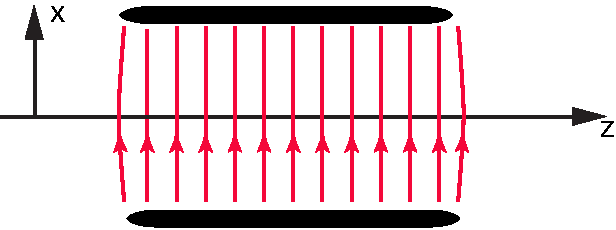
\includegraphics[width=5in]{elseparator.pdf}
  \caption[ElSeparator electric field.]
  {
Elseparator Electric field. The fringe field lines break the
translational invariance in $x$.
  }
  \label{f:elsep}.
\end{figure}

[Thanks to \'Etienne Forest for the derivation of the elseparator equation of motion.]

The Hamiltonian for an electric separator is 
\Begineq
  H = -p_s 
  = - \left\{ \left( \frac{1}{\beta_0} + \delta + k_E \, x \right)^2 - 
  \wt m^2 - p_x^2 - p_y^2 \right\}^{1/2}
  \label{hp1b}
\Endeq
Here the canconical coordinates $(-c \, t, \delta$ are being used,
$\wt m$ is defined in \Eq{mmccp}, and $p_s = -H$ is just the
longitudinal momentum.  In the above equation, $k_E$ is the normalized
field
\Begineq
  k_E = \frac{q \, E}{P_0 \, c}
\Endeq
The field is taken to be pointing along the $x$-axis with positive
$k_E$ accelerating a particle in the positive $x$ direction. To solve
the equations of motion, a ``hard edge'' model is used where $k_E$ is
constant inside the separator and the field ends abrouptly at the
separator edges.

\index{solenoid}
Since, as shown in \fig{f:elsep}, the fringe fields break the
translational invariance in $x$, it is important here that the $x = 0$
plane be centered within the separator plates. With this, the
canonical momentum $\delta$ just outside the separator assumes its
free space form of $\delta = (E - E_0) / E_0)$. This is analogous to
the case of a \vn{solenoid} where, to ensure that the canonical
transverse momenta assume their free space form just outside the
solenoid, the $\Bf z$-axis must be along the centerline of the
solenoid.

The solution of the equations of motion is:
\begin{align}
  x   &= (x_0 - x_c) \, \cosh \left( \frac{k_E \, L}{p_s} \right) + 
         \frac{p_{x0}}{k_E} \, \sinh \left( \frac{k_E \, L}{p_s} \right) + x_c \CRNO
  p_x &= k_E \, (x_0 - x_c) \, \sinh \left( \frac{k_E \, L}{p_s} \right) + 
         {p_{x0}} \, \cosh \left( \frac{k_E \, L}{p_s} \right) \CRNO
  y   &= y_0 + L \, \frac{p_{y0}}{p_s} \label{xxlp} \\
  p_y &= p_{y0} \CRNO
  c \, \delta t &=  \int_0^L -\frac{\partial H}{\partial \delta}
      = (x_0 - x_c) \, \sinh \left( \frac{k_E \, L}{p_s} \right) +
        \frac{p_{x0}}{k_E} \, \left[ \cosh \left( \frac{k_E \, L}{p_s} \right) - 1 \right]
        \nonumber
\end{align}
where the critical position $x_c$ is
\Begineq 
  x_c = -\frac{\wt E}{k_E}
\Endeq
and 
\Begineq
  \wt E \equiv \frac{1}{\beta_0} + \delta = \frac{E}{P_0 \, c}
\Endeq
 
\Eqs{xxlp} predict that for $x < x_c$ and $p_{x0} = 0$ a particle
will, unphysically, accelerate in the negative $x$ direction. In
actuality, a particle in this instance will be reflected backwards by
the longitudinal component of the edge field. Specifically, the
argument of the square root in \Eq{hp1b} must be non-negative and
a particle will only make it through the speparator if
\Begineq
  x_0 > \frac{1}{k_E} \, \left( \sqrt{\wt m^2 + p_{x0}^2 + p_{y0}^2} - \wt E \right)
\Endeq

%---------------------------------------------------------------------------------
%---------------------------------------------------------------------------------
\section{Kicker, Hkicker, and Vkicker, Tracking}
\label{s:kicker.std}
\index{kicker}
\index{hkicker}
\index{vkicker}
\index{elseparator}

The Hamiltonian for a horizontally deflecting kicker or separator is
\Begineq
  H = \frac{p_x^2 + p_y^2}{2 (1 + p_z)} - k_0 \, x 
\Endeq
This gives the map
\begin{align}
  x_2    &= x_1 + \frac{1}{1 + p_{z1}} \, \left( L \, p_{x1} + \frac{1}{2} k_0 \, L^2 \right) \CRNO
  p_{x2} &= p_{x1} + k_0 \, L \CRNO
  y_2    &= y_1 + \frac{L \, p_{y1}}{1 + p_{z1}} \CRNO
  p_{y2} &= p_{y1}  \\
  z_2    &= z_1 - \frac{L}{2 (1 + p_{z1})^2} \, 
    \left( p_{x1}^2 + p_{y1}^2 + p_{x1} \, k_0 \, L + \frac{1}{3} k_0^2 \, L^2 \right) \CRNO
  p_{z2} &= p_{z1} \nonumber
\end{align}
The generalization when the kick is not in the horizontal plane is easily derived.

%---------------------------------------------------------------------------------
%---------------------------------------------------------------------------------
\section{Lcavity Tracking}
\label{s:lcavity.std}
\index{lcavity}

The transverse trajectory through an \vn{Lcavity} is modeled using equations
developed by Rosenzweig and Serafini\cite{b:rosenzweig} (R\&S) with
\begin{align}
  b_0 &= 1 \CRNO
  b_{-1} &= 1 
\end{align}
and all other $b_n$ set to zero.

The transport equations in R\&S were developed in the
ulta-relativistic limit with $\beta = 1$.  To extend these equations,
the transport through the cavity body (R\&S Eq.~(9)) has been modified
to give the correct phase-space area at non ultra-relativistic
energies:
\Begineq
  \begin{pmatrix}
    x \\ 
    x'
  \end{pmatrix}_2 = 
  \begin{pmatrix}
    \cos(\alpha)  &  
    \sqrt{\frac{8}{\eta(\Delta\phi)}} \, \frac{\beta_1 \, \gamma_1}{\gamma'} \, 
                                                   \cos(\Delta\phi) \, \sin(\alpha) \\
    -\sqrt{\frac{\eta(\Delta\phi)}{8}} \, 
                     \frac{\gamma'}{\beta_2 \, \gamma_2 \, \cos(\Delta\phi)} \, \sin(\alpha) &
    \frac{\beta_1 \, \gamma_1}{\beta_2 \, \gamma_2} \, \cos(\alpha)
  \end{pmatrix}
  \,
  \begin{pmatrix}
    x \\ 
    x'
  \end{pmatrix}_1
\Endeq
The added factors of $\beta$ give the matrix the correct determinate
of $\beta_1 \, \gamma_1 / \beta_2 \, \gamma_2$. {\em While the added
factors of $\beta$ do correct the phase space area, the above equation
can only be considered as a rough approximation for simulating
particles when $\beta$ is significantly different from 1. Indeed, the
only accurate way to simulate such particles is by integrating through
the actual field [Cf.~Runge Kutta tracking (\sref{s:tkm})]}

The change in $z$ going through a cavity is calculated by first calculating the particle
transit time $\Delta t$
\begin{align}
  c \, \Delta t &= \int_{s_1}^{s_2} \!\! ds \,\, \frac{1}{\beta(s)} \CRNO
  &= \int_{s_1}^{s_2} \!\! ds \, \frac{E}{\sqrt{E^2 - (mc^2)^2}} \\
  &= \frac{c \, P_{z2} - c \, P_{z1}}{G} \nonumber
\end{align}
where it has been assumed that the accelerating gradient $G$ is
constant through the cavity. In this equation $\beta = v / c$, $E$ is
the energy, and $P_{z1}$ and $P_{z2}$ are the entrance and exit
momenta. Using \Eq{zbctt}, the change in $z$ is thus
\Begineq
  z_2 = \frac{\beta_2}{\beta_1} \, z_1 - 
  \beta_2 \, 
  \left(
  \frac{c \, P_{z2} - c \, P_{z1}}{G} - 
  \frac{c \, \Pbar_{z2} - c \, \Pbar_{z1}}{\BAR G}
  \right)
\Endeq
where $\Pbar$ and $\BAR G$ are the momentum and gradient of the
reference particle.

Note that the above transport equations are only symplectic on-axis
There are second order terms in the transverse coordinates that are
missing. To obtain a proper symplectic matrix, the \vn{symplectify}
attirubte of an \vn{lcavity} element (\sref{s:symp}) can be set to
True.

%---------------------------------------------------------------------------------
%---------------------------------------------------------------------------------
\section{Mirror Tracking}
\label{s:mirror.std}
\index{mirror}

%---------------------------------------------------------------------------------
%---------------------------------------------------------------------------------
\section{Octupole Tracking}
\label{s:octupole.std}
\index{octupole}

The Hamiltonian for an upright octupole is
\Begineq
  H = \frac{p_x^2 + p_y^2}{2 (1 + p_z)} + \frac{k_3}{24} (x^4 - 6 \, x^2 \, y^2 + y^4)
\Endeq

An octupole is modeled using a kick-drift-kick model.

%---------------------------------------------------------------------------------
%---------------------------------------------------------------------------------
\section{Patch Tracking}
\label{s:patch.std}
\index{patch}

\begin{figure}[tb]
  \centering
  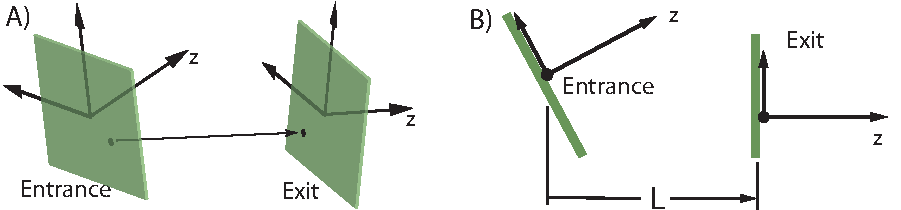
\includegraphics[width=5in]{patch.pdf}
  \caption[Standard patch transformation.]
{Standard tracking through a patch element. A particle's starting coordinate at
the entrance end of the patch has, by construction, coordinate $z$ =
0. The particle is drifted, as in a field free region, between the
entrance $z = 0$ plane and the exit $z = 0$ plane.}
  \label{f:patch.track}
\end{figure}

%---------------------------------------------------------------------------------

The transformation of the reference coordinates through a ``standard''
patch (a patch where custom fields are not used) is given by
\Eqs{vwlv} and \eq{wws}. At the entrance end of the patch, a
particle's position and momentum in the entrance coordinate system will be
\begin{alignat}{1}
  \bfr &= (x, y, 0) \CRNO
  \bfP &= (P_x, P_y, P_z) = 
    \left( p_x, p_y, \pm \sqrt{(1+p_z)^2 - p_x^2 - p_y^2} \right) \, P_{0\text{ent}}
\end{alignat}
where $p_x$, $p_y$ and $p_z$ are the phase space momenta, and $z$,
which is coordinate $z$ and not phase space $z$, is always zero by
construction as shown in \fig{f:patch.track} [Also see \fig{f:local.coords}
and the discussion in \sref{s:phase.space}.] The sign of the
longitudinal momentum $P_z$ is determined by whether the particle is
traveling in the positive $s$ or negative $s$ direction (which will
occur when an element is flipped longitudinally).

The transformation between entrance and exit coordinate systems is given by \Eqs{rwlr} and \eq{pps}
\begin{alignat}{1}
  \bfr &\rightarrow 
    \bfS^{-1} \, (\bfr - \bfL_\text{off}) \CRNO
  \bfP &\rightarrow \bfS^{-1} \, \bfP
\end{alignat}
where $\bfL_\text{off}$ is given by \Eq{swww}

After this transformation, the particle must be propagated by a longitudinal length
$-r_z$ to intersect the $r_z = 0$ plane of the exit face.
\begin{alignat}{1}
  \bfr &\rightarrow (r_x - r_z \, \frac{P_x}{P_z}, r_y - r_z \, \frac{P_y}{P_z}, 0) \CRNO
  \bfP &\rightarrow \bfP
\end{alignat}

The final $\bfr$ and $\bfP$ can now be used compute the particles
phase space coordinates, along with the time $t$ and the reference time
$t_{\text{ref}}$ at the exit end.
\begin{alignat}{3}
  x &\rightarrow r_x \qquad &p_x &\rightarrow \frac{P_x}{P_{0\text{exi}}} \CRNO
  y &\rightarrow r_y \qquad &p_y &\rightarrow \frac{P_y}{P_{0\text{exi}}} \\
  z &\rightarrow z + r_z \, \frac{|\bfP|}{P_z} + L_0 \, \frac{\beta}{\beta_0} +
    \beta \, \text{t_offset} \qquad
    &p_z &\rightarrow \frac{(1+p_z) \, P_{0\text{ent}} - P_{0\text{exi}}}{P_{0\text{exi}}} \CRNO
  t &\rightarrow t - r_z \, \frac{|\bfP|}{P_z \, \beta} \qquad
  &t_{\text{ref}} &\rightarrow t_{\text{ref}} + \text{t_offset} + L_0 \, \frac{1}{\beta_0} \nonumber
\end{alignat}
where the exit reference momentum $P_{0\text{exi}}$ is related to the
entrance reference momentum $P_{0\text{ent}}$ through
\vn{e_tot_offset}.  In the above equation, $\beta$ is the particle
velocity, $\beta_0$ is the velocity of the reference particle, and
$L_0$ is the drift length of the reference particle
\Begineq
  L_0 = \frac{1}{S^{-1}_{33}} \, \left( 
  S^{-1}_{31} \, \text{x_offset} + S^{-1}_{32} \, \text{y_offset} + S^{-1}_{33} \, \text{z_offset}
  \right)
\Endeq

%---------------------------------------------------------------------------------
%---------------------------------------------------------------------------------
\section{Quadrupole Tracking}
\label{s:quadrupole.std}
\index{quadrupole}

The \vn{bmad_standard} calculates the transfer map through an upright
quadrupole and then transforms that map to the laboratory frame.

The Hamiltonian for an upright quadrupole is
\Begineq
  H = \frac{p_x^2 + p_y^2}{2 (1 + p_z)} + \frac{k_1}{2} (x^2 - y^2)
\Endeq
This is simply solved
\begin{align}
  x_2    &= c_x \, x_1 + s_x \, \frac{p_{x1}}{1 + p_{z1}} \CRNO
  p_{x2} &= \tau_x \, \om^2 \, \, (1 + p_{z1}) \, s_x \, x_1 + c_x \, p_{x1} \CRNO
  y_2    &= c_y \, y_1 + s_y \, \frac{p_{y1}}{1 + p_{z1}} \CRNO
  p_{y2} &= \tau_y \, \om^2 \, \, (1 + p_{z1}) \, s_y \, y_1 + c_y \, p_{y1} \\
  z_2    &= z_1 + m_{511} \, x_1^2 + m_{512} \, x_1 \, p_{x1} + m_{522} \, p_{x1}^2 + 
                   m_{533} \, y_1^2 + m_{534} \, y_1 \, p_{y1} + m_{544} \, p_{y1}^2 \CRNO
  p_{z2} &= p_{z1} \nonumber
\end{align}
where 
\Begineq
  \om \equiv \sqrt{\frac{|k_1|}{1 + p_{z1}}}
\Endeq
and
\begin{alignat}{6}
         &\hspace*{3ex}  && k_1 > 0          &\hspace*{3ex}& k_1 < 0 & \qqquad
         &\hspace*{3ex}  && k_1 > 0          &\hspace*{3ex}& k_1 < 0 \CRNO
     c_x &=   && \cos  (\om \, L) && \cosh (\om \, L) & \qqquad
     c_y &=   && \cosh (\om \, L) && \cos  (\om \, L) \CRNO
     s_x &=   && \frac{\sin  (\om \, L)}{\om} && \frac{\sinh (\om \, L)}{\om} & \qqquad
     s_y &=   && \frac{\sinh (\om \, L)}{\om} && \frac{\sin  (\om \, L)}{\om} \\
  \tau_x &=   && {-}1             && {+}1             & \qqquad
  \tau_y &=   && {+}1             && {-}1             \nonumber
\end{alignat}
with this
\begin{alignat}{2}
  m_{511} &= \frac{\tau_x \,\, \om^2}{4} \, (L - c_x \, s_x) & \qqquad
  m_{533} &= \frac{\tau_y \,\, \om^2}{4} \, (L - c_y \, s_y) \CRNO
  m_{512} &= \frac{-\tau_x \,\, \om^2}{2 \, (1 + p_{z1})} \, s_x^2 & \qqquad
  m_{534} &= \frac{-\tau_y \,\, \om^2}{2 \, (1 + p_{z1})} \, s_y^2 \\
  m_{522} &= \frac{-1}{4 \, (1 + p_{z1})^2} \, (L + c_x \, s_x) & \qqquad
  m_{544} &= \frac{-1}{4 \, (1 + p_{z1})^2} \, (L + c_y \, s_y) \nonumber
\end{alignat}

%---------------------------------------------------------------------------------
%---------------------------------------------------------------------------------
\section{RFcavity Tracking}
\label{s:rfcavity.std}
\index{rfcavity}

Tracking through an rfcavity uses a kick-drift-kick model. The kick is
a pure energy kick (see equations in \sref{s:rfcav}) and the phase of
the RF is calculated under the assumption that the waveform moves at a
phase velocity equal to the velocity of the reference particle.

\index{lcavity}
The transverse forces due to the RF are ignored. This is a resonable
approximation when the acceleration is small. \vn{Lcavity} elements
should be used in place of \vn{rfcavity} elements when this is not so.

%---------------------------------------------------------------------------------
%---------------------------------------------------------------------------------
\section{Sad\_Mult Tracking}
\label{s:sad.mult.std}
\index{sad_mult}

The ``hard edge'' fringe field kick is taken from Forest\cite{b:forest} Eqs.~(13.29) and onward.
In the notation of \bmad, and taking into account both normal and skew terms, Eq.~(13.29)
is for the $m$\th order multipole (what Forest labels $n+1$)
\Begineq
  f_\pm = \mp \Re \frac{(b_m + i \, a_m) \, (x + i \, y)^{(m+1)}}{4 \, (m+2) \, (1 + p_z)}
    \left[ x \, p_x + y \, p_y + i\frac{m+3}{m+1}(x \, p_y - y \, p_x) \right]
\Endeq

The ``soft edge'' dipole fringe for \vn{sad_mult} elements is a generalization of the soft edge
dipole fringe for a SAD bend element. For the entrance kick the equations are:
\begin{align}
  x_2 &= x_1 + \frac{\delta_1}{1 + \delta_1} \, \Delta x_{fx}, \qquad
  p_{x2} = p_{x1} + \frac{1}{1 + \delta_1} \, \left[ 
    \Delta x_{fy} \, v - \Delta x_{fay} \, v^3 \right] \CRNO
  y_2 &= y_1 - \frac{\delta_1}{1 + \delta_1} \, \Delta y_{fy}, \qquad
  p_{y2} = p_{y1} + \frac{1}{1 + \delta_1} \, \left[ 
    \Delta y_{fx} \, w - \Delta y_{fax} \, w^3 \right] \\
  z_2 &= z_1 + \frac{1}{(1 + \delta_1)^2} \, \left[ \, 
    \Delta x_{fx} \, p_{x1} - \Delta y_{fy} \, p_{y1} + 
    \frac{1}{2} \, (\Delta y_{fx} + \Delta x_{fy}) \, w^2 -
    \frac{1}{4} (\Delta y_{fax} + \Delta x_{fay}) \, w^4
    \right] \nonumber
\end{align}
where
\begin{alignat}{3}
  \Delta x_{fx}  &= \frac{K_0 \, F_B^2}{24 \, L}, & \qquad 
  \Delta y_{fx}  &= \frac{K_0^2 \, F_B}{6 \, L^2}, & \qquad 
  \Delta y_{fax} &= \frac{2 \, K_0^2}{3 \, F_B \, L^2}, \CRNO 
  \Delta y_{fy}  &= \frac{SK_0 \, F_B^2}{24 \, L}, & \qquad
  \Delta x_{fy}  &= \frac{SK_0^2 \, F_B}{6 \, L^2}, & \qquad
  \Delta x_{fay} &= \frac{2 \, SK_0^2}{3 \, F_B \, L^2}, \\
  v &= \cos\theta \, x_1 + \sin\theta \, y_1, & \qquad
  w &= -\sin\theta \, x_1 + \cos\theta \, y_1, & \qquad
  \tan\theta &= \frac{-SK_0}{K_0} \nonumber
\end{alignat}


%---------------------------------------------------------------------------------
%---------------------------------------------------------------------------------
\section{Sextupole Tracking}
\label{s:sextupole.std}
\index{sextupole}

The Hamiltonian for an upright sextupole is
\Begineq
  H = \frac{p_x^2 + p_y^2}{2 (1 + p_z)} + \frac{k_2}{6} (x^3 - 3 \, x \, y^2)
\Endeq

Tracking through a sextupole uses a kick-drift-kick model.

%---------------------------------------------------------------------------------
%---------------------------------------------------------------------------------
\section{Sol\_Quad Tracking}
\label{s:sol.quad.std}
\index{sol_quad}

The Hamiltonian is
\Begineq
  H = \frac{(p_x + \frac{k_s }{2}\, y)^2}{2 (1 + p_z)} + 
  \frac{(p_y - \frac{k_s}{2} \, x)^2}{2 (1 + p_z)} + \frac{k_1}{2} (x^2 - y^2)
\Endeq
Solving the equations of motion gives
\begin{align}
  x_2    &= m_{11} \, x_1 + m_{12} \, p_{x1} + m_{13} \, y_1 + m_{14} \, p_{y1} \CRNO
  p_{x2} &= m_{21} \, x_1 + m_{22} \, p_{x1} + m_{23} \, y_1 + m_{24} \, p_{y1} \CRNO
  y_2    &= m_{31} \, x_1 + m_{32} \, p_{x1} + m_{33} \, y_1 + m_{34} \, p_{y1} \CRNO
  p_{y2} &= m_{41} \, x_1 + m_{42} \, p_{x1} + m_{43} \, y_1 + m_{44} \, p_{y1} \\
  z_2    &= z_1 + \sum_{j = 1}^4 \sum_{k = j}^4 m_{5jk} \, r_j \, r_k  \CRNO
  p_{z2} &= p_{z1} \nonumber
\end{align}
where
\begin{alignat}{2}
  m_{11} &= \frac{1}{2 \, f} \, \left( f_{0+} \, c + f_{0-} \, c_h \right) & \qqquad
  m_{31} &= -m_{24} \CRNO
  m_{12} &= \frac{1}{2 \, f \, (1 + p_{z1})} \, 
            \left( \frac{f_{++}}{\om_+} \,  s + \frac{f_{--}}{\om_-} \, s_h \right) & \qqquad
  m_{32} &= -m_{14} \CRNO
  m_{13} &= \frac{\ks}{4 \, f} \, 
            \left( \frac{f_{+-}}{\om_+} \, s +\frac{f_{-+}}{\om_-} \, s_h \right) & \qqquad
  m_{33} &= \frac{1}{2 \, f} \, \left( f_{0-} \, c + f_{0+} \, c_h \right) \CRNO
  m_{14} &= \frac{\ks}{f \, (1 + p_{z1})} \, \left( -c + c_h \right) & \qqquad
  m_{34} &= \frac{1}{2 \, f \, (1 + p_{z1})} \, 
            \left( \frac{f_{+-}}{\om_+} \, s + \frac{f_{-+}}{\om_-} \, s_h \right) \CRNO
  m_{21} &= \frac{-(1 + p_{z1})}{8 \, f} \, 
            \left( \frac{\xi_{1+}}{\om_+} \, s + \frac{\xi_{2+}}{\om_-} s_h \right) & \qqquad
  m_{41} &= -m_{23} \\
  m_{22} &= m_{11} & \qqquad
  m_{42} &= -m_{13} \CRNO
  m_{23} &= \frac{\ks^3 \, (1 + p_{z1})}{4 \, f} \, \left( c - c_h \right) & \qqquad
  m_{43} &= \frac{-(1 + p_{z1})}{8 \, f} \, 
            \left( \frac{\xi_{1-}}{\om_+} \, s + \frac{\xi_{2-}}{\om_-} \, s_h \right) \CRNO
  m_{24} &= \frac{\ks}{4 \, f} \, 
            \left( \frac{f_{++}}{\om_+} \, s + \frac{f_{--}}{\om_-} \, s_h \right) & \qqquad
  m_{44} &= m_{33} \nonumber
\end{alignat}
and
\begin{alignat}{2}
  \kone        &= \frac{k_1}{1 + p_{z1}} & \qqquad 
  \ks          &= \frac{k_s}{1 + p_{z1}} \CRNO
  f            &= \sqrt{\ks^4 + 4 \, \kone^2} & \qqquad
  f_{\pm0}     &= f \pm \ks^2 \CRNO
  f_{0\pm}     &= f \pm 2 \, \kone & \qqquad
  f_{\pm\pm}   &= f \pm \ks^2 \pm 2 \, \kone \CRNO
  \om_+        &= \sqrt{\frac{f_{+0}}{2}} & \qqquad
  \om_-        &= \sqrt{\frac{f_{-0}}{2}} \\
  s            &= \sin (\om_+ \, L) & \qqquad
  s_h          &= \sinh (\om_- \, L) \CRNO
  c            &= \cos (\om_+ \, L) & \qqquad
  c_h          &= \cosh (\om_- \, L) \CRNO
  \xi_{1\pm} &= \ks^2 \, f_{+\mp} \pm 4 \, \kone \, f_{+\pm} & \qqquad
  \xi_{2\pm} &= \ks^2 \, f_{-\pm} \pm 4 \, \kone \, f_{-\mp} \nonumber
\end{alignat}

The $m_{5jk}$ terms are obtained via \Eq{zz121p}
\begin{align}
  m_{5jk} = - \frac{\tau_{jk}}{2 (1 + p_{z1})^2} \int \! ds \, 
  & \left[ 
    \left( m_{2j} + \frac{k_s}{2} \, m_{3j} \right) \, 
    \left( m_{2k} + \frac{k_s}{2} \, m_{3k} \right)   
  \right. + \\
  & \hspace*{15ex} \left.
    \left( m_{4j} - \frac{k_s}{2} \, m_{1j} \right) \, 
    \left( m_{4k} - \frac{k_s}{2} \, m_{1k} \right) 
  \right] \nonumber
\end{align}
where
\Begineq
  \tau_{jk} = 
  \begin{cases}
    1 & j = k \\
    2 & j \ne k 
  \end{cases}
\Endeq
The needed integrals involve the product of two trigonometric or
hyperbolic functions. These integrals are trivial to do but the
explicit equations for $m_{5jk}$ are quite long and in the interests of
brevity are not reproduced here.

%---------------------------------------------------------------------------------

\begin{figure}[tb]
  \centering
  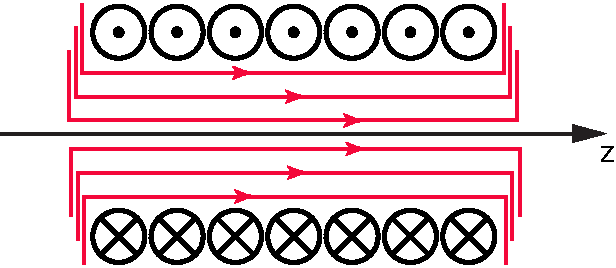
\includegraphics[width=5in]{solenoid.pdf}
  \caption[Solenoid with a hard edge.]
  {
Solenoid with a hard edge. The field is assumed to end abruptly at the
edges of the solenoid. Here, for purposes of illustration, the field lines at
the ends are displaced from one another.
  }
  \label{f:solenoid}.
\end{figure}

%---------------------------------------------------------------------------------
%---------------------------------------------------------------------------------
\section{Solenoid Tracking}
\label{s:solenoid.std}
\index{solenoid}

The Hamiltonian for a solenoid is
\Begineq
  H = \frac{ \left( p_x + \frac{k_s}{2} \, y \right)^2}{2 \, (1 + p_z)} + 
  \frac{ \left( p_y - \frac{k_s}{2} \, x \right)^2}{2 \, (1 + p_z)} 
\Endeq
where the normalized field $k_s$ is
\Begineq
  k_s = \frac{B}{P_0}
\Endeq
The solution to the equations of motion for a constant $k_s$ are
\begin{align}
  x_2    &= \frac{1 + c}{2} \, x_1 + \frac{s}{k_s} \, p_{x1} +
           \frac{s}{2} \, y_1 + \frac{1 - c}{k_s} \, p_{y1} \CRNO
  p_{x2} &= \frac{-k_s \, s}{4} \, x_1 + \frac{1 + c}{2} \, p_{x1} - 
           \frac{k_s \, (1 - c)}{4} \, y_1 + \frac{s}{2} \, p_{y1} \CRNO
  y_2    &= \frac{-s}{2} \, x_1 - \frac{1 - c}{k_s} \, p_{x1} +
           \frac{1 + c}{2} \, y_1 + \frac{s}{k_s} \, p_{y1} \\      
  p_{y2} &= \frac{k_s \, (1 - c)}{4} \, x_1 + \frac{-s}{2} \, p_{x1} -
            \frac{k_s \, s}{4} \, y_1 + \frac{1 + c}{2} \, p_{y1} \CRNO 
  z_2    &= z_1 + \frac{L}{2 \, (1 + p_{z1})^2} \, 
                   \left[ \left( p_{x1} + \frac{k_s}{2} \, y_1 \right)^2 +
                          \left( p_{y1} - \frac{k_s}{2} \, x_1 \right)^2 \right] \CRNO
  p_{z2} &= p_{z1} \nonumber
\end{align}
where
\begin{align}
  c &= \cos \left( \frac{k_s}{2} \, L \right) \CRNO
  s &= \sin \left( \frac{k_s}{2} \, L \right)
\end{align}

To be useful, the canonical momenta $p_x$ and $p_y$ in the above
equations must be connected to the cononical momenta used for other
elements (drifts, quadrupoles, etc.) that may be placed to either side
of the solenoid. These side elements use zero $a_x$ and $a_y$
(cf. \Eq{pmc2pc}). The vector potential used in the solenoid canonical
momenta may be made zero at the edges of the solenoid if the solenoid
fringe field is assumed to end abruptly at the edges of the solenoid
(as shown in \fig{f:solenoid}), and the reference axis $\Bf z$-axis (at
$x$ = $y$ = 0) is placed along the centerline of the solenoid so that
there is cylendrical symmetry around the $\Bf z$-axis.

%---------------------------------------------------------------------------------
\section{Symplectic Tracking with Cartesian Modes}
\label{s:wiggler.std}
\index{wiggler!tracking}

The method for symplectic integration for elements that define the magnetic field using a
Cartesian mode decomposition (\sref{s:cart.map}) is outlined in \sref{s:symp.track}.  The
vector potential is constructed to avoid singularities when one of the wave vectors $k_x$,
$k_y$, or $k_z$ is zero.

For the \vn{x} \vn{family} the vector potential is:
\begin{center}
{
\setlength{\tabcolsep}{1pt}
\begin{tabular}{lrllrllrll}
  Form \; & \multicolumn{3}{l}{hyper-y}  & \multicolumn{3}{l}{hyper-xy}  & \multicolumn{3}{l}{hyper-x} \\
  $A_x$   & 
    $A$ & $\dfrac{k_z}{k_y^2}$      & $\Se_x \, \Sh_y \, \Se_z \qquad$ &
    $A$ & $\dfrac{1}{k_y}$          & $\Sh_x \, \Sh_y \, \Se_z \qquad$ &
    $A$ & $\dfrac{k_z}{k_x \, k_y}$ & $\Sh_x \, \Se_y \, \Se_z$ \\
  $A_y$   & 0 &&& 0 &&& 0 && \\
  $A_z$   & 
    $A$ & $\dfrac{k_x}{k_y^2}$      & $\Ce_x \, \Sh_y \, \Ce_z \qquad$ &
    $A$ & $\dfrac{k_x}{k_y \, k_z}$ & $\Ch_x \, \Sh_y \, \Ce_z \qquad$ &
    $A$ & $\dfrac{1}{k_y}$          & $\Ch_x \, \Se_y \, \Ce_z$ 
\end{tabular}
}
\end{center}

For the \vn{y} \vn{family} the vector potential is:
\begin{center}
{
\setlength{\tabcolsep}{1pt}
\begin{tabular}{lrllrllrll}
  Form \; & \multicolumn{3}{l}{hyper-y}  & \multicolumn{3}{l}{hyper-xy}  & \multicolumn{3}{l}{hyper-x} \\
  $A_x$   & 0 &&& 0 &&& 0 && \\
  $A_y$   & 
    $-A$ & $\dfrac{k_z}{k_x \, k_y}$ & $\Se_x \, \Sh_y \, \Se_z \qquad$ &
    $-A$ & $\dfrac{1}{k_x}$          & $\Sh_x \, \Sh_y \, \Se_z \qquad$ &
    $-A$ & $\dfrac{k_z}{k_x^2}$      & $\Sh_x \, \Se_y \, \Se_z$ \\
  $A_z$   & 
    $-A$ & $\dfrac{1}{k_x}$          & $\Se_x \, \Ch_y \, \Ce_z \qquad$ &
    $-A$ & $\dfrac{k_y}{k_x \, k_z}$ & $\Sh_x \, \Ch_y \, \Ce_z \qquad$ &
    $-A$ & $\dfrac{k_y}{k_x^2}$      & $\Sh_x \, \Ce_y \, \Ce_z$ 
\end{tabular}
}
\end{center}

For the \vn{qu} \vn{family} the vector potential is:
\begin{center}
{
\setlength{\tabcolsep}{1pt}
\begin{tabular}{lrllrllrll}
  Form \; & \multicolumn{3}{l}{hyper-y}  & \multicolumn{3}{l}{hyper-xy}  & \multicolumn{3}{l}{hyper-x} \\
  $A_x$   & 
     $A$ & $\dfrac{1}{k_z}$          & $\Se_x \, \Ch_y \, \Se_z \qquad$ &
     $A$ & $\dfrac{k_y}{k_z^2}$      & $\Sh_x \, \Ch_y \, \Se_z \qquad$ &
     $A$ & $\dfrac{k_y}{k_x \, k_z}$ & $\Sh_x \, \Ce_y \, \Se_z$ \\
  $A_y$   & 
    $-A$ & $\dfrac{k_x}{k_y \, k_z}$ & $\Ce_x \, \Sh_y \, \Se_z \qquad$ &
    $-A$ & $\dfrac{k_x}{k_z^2}$      & $\Ch_x \, \Sh_y \, \Se_z \qquad$ &
    $-A$ & $\dfrac{1}{k_z}$          & $\Ch_x \, \Se_y \, \Se_z$ \\
  $A_z$   & 0 &&& 0 &&& 0 &&
\end{tabular}
}
\end{center}

For the \vn{sq} \vn{family} the vector potential is:
\begin{center}
{
\setlength{\tabcolsep}{1pt}
\begin{tabular}{lrllrllrll}
  Form \; & \multicolumn{3}{l}{hyper-y}  & \multicolumn{3}{l}{hyper-xy}  & \multicolumn{3}{l}{hyper-x} \\
  $A_x$   & 
     $A$ & $\dfrac{1}{k_z}$          & $\Ce_x \, \Sh_y \, \Se_z \qquad$ &
     $A$ & $\dfrac{k_y}{k_z^2}$      & $\Ch_x \, \Sh_y \, \Se_z \qquad$ &
     $A$ & $\dfrac{k_y}{k_x \, k_z}$ & $\Ch_x \, \Se_y \, \Se_z$ \\
  $A_y$   & 
     $A$ & $\dfrac{k_x}{k_y \, k_z}$ & $\Se_x \, \Ch_y \, \Se_z \qquad$ &
    $-A$ & $\dfrac{k_x}{k_z^2}$      & $\Sh_x \, \Ch_y \, \Se_z \qquad$ &
     $A$ & $\dfrac{1}{k_z}$          & $\Sh_x \, \Ce_y \, \Se_z$ \\
  $A_z$   & 0 &&& 0 &&& 0 &&
\end{tabular}
}
\end{center}

